\chapter{Implementation}
\label{cha:implementation}

In the chapter we explain how the implementation is done for both the frontend and the backend sides.
We first elaborate on the different roles exist in the frontend:

\section{Frond-end}

\textbf{IDE}: Visual Studio code\\
\textbf{Language}: React\\
\textbf{Libraries used}:
\begin{itemize}
    \item react-router-dom
    \item receiver mail must be a register user
\end{itemize}


\subsection{Costumer}
Libraries used:
\begin{itemize}
\item rc-slider for creating the tempatrue slide bar 
\item react-horizontal-timeline for the time line
\item redux-form for the registration form
\end{itemize}

The costumer role refer to any individual who send a package through the system.
The costumer has the following abilities:

\begin{itemize}
    \item register a package
    \item delete a package
    \item show a package detail view 
    \item time line
\end{itemize}


\subsubsection{Register a package}
The register package process divided by two component:
\begin{itemize}
\item RegisterPackage.js - view (child)
\item UserSpace.js - controller (father)
\end{itemize}


\begin{figure}[!ht]
	\centering
	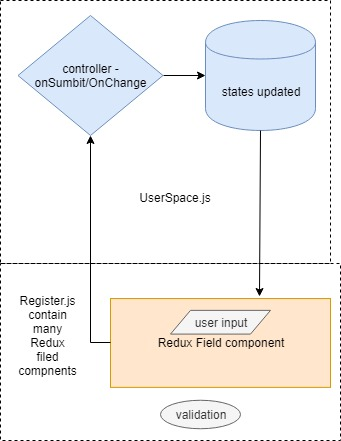
\includegraphics[width=0.5\textwidth]{images/register.jpg}
	\caption{register package process, component diagram}
	\label{fig:}
\end{figure}


The component ResgiterPackage is an assembly of Redux <Field> component and React input.
for each input field the user enter, the page is rendered and the state is updated
The form contain the following validation:
\begin{itemize}
\item no text input filed can be left empty 
\item receiver mail must be a register user
\end{itemize}
i.e without standing in the form requirement, the user can not press the submit button.

When registering a package, a sensor data may be provided by clicking the correspond checkbox. It is import to mention that not every package has a sensors data.\\
HTTP requests arrive from the browser at the backend are integral part to insure system operation
After pressing the sumbit button the following occures:\\
1. \textbf{http://localhost:8000/address} post request to enter the address and get back and ID for each user\\
2. \textbf {http://localhost:8000/packages}  post request to enter the packages to the packages tables, return a package \\
3. \textbf {http://localhost:8000/OrderSensors}  post request to enter the sensors (if exist)  to the sensore table, return a sensore id\\
4.\textbf {http://localhost:8000/OrderHistory}  post request to enter the action(registration) as part of the order history for later on use in the time-line\\

\subsubsection{cancel package}
The feature cancel package allows the user to delete a cancel package.
After pressing the navbar "delete package" option, the user will be directed to the Activs.js compnent.\newline
The user will be shown only packages in a "register" status, \textbf{any other package which has being dispatch already can not be cancel}.\newline
From the system perspective while the package is being canceled, the data is not deleted from storage,it will only be marked as canceled. algorithm:
\begin{enumerate}
  \item \textbf{http://localhost:8000/packages/user/}  get request before component moount: upload all packages with "register" status
  \item if user press delete:
  \begin{enumerate}
      \item textbf {http://localhost:8000/packages/:id}  put request to change the spesific package to "cancel" mode.
      \item textbf {http://localhost:8000/OrderHistory}  post reqest. update the timeline, add the event to history
\end{enumerate}
\end{enumerate}